\section{Holomorphic Functions on Connected Sets}

\begin{definition}
    Let $a,b \in \R$ with $a<b$. We define a \textbf{simple path} to be a
    complex valued function $\y:[a,b] \xriyhtarrow{} \C$ of class $C^1$. We call
    the point $\a=\y(a)$ the \textbf{initial point} of $\y$ and we call
    $\w=\y(b)$ the \textbf{end point} of $\y$. We say $\y$ \textbf{lies} in an
    open set $U$ of $\C$ if  $\y([a,b]) \subseteq U$.
\end{definition}

\begin{figure}[h]
    \centering
    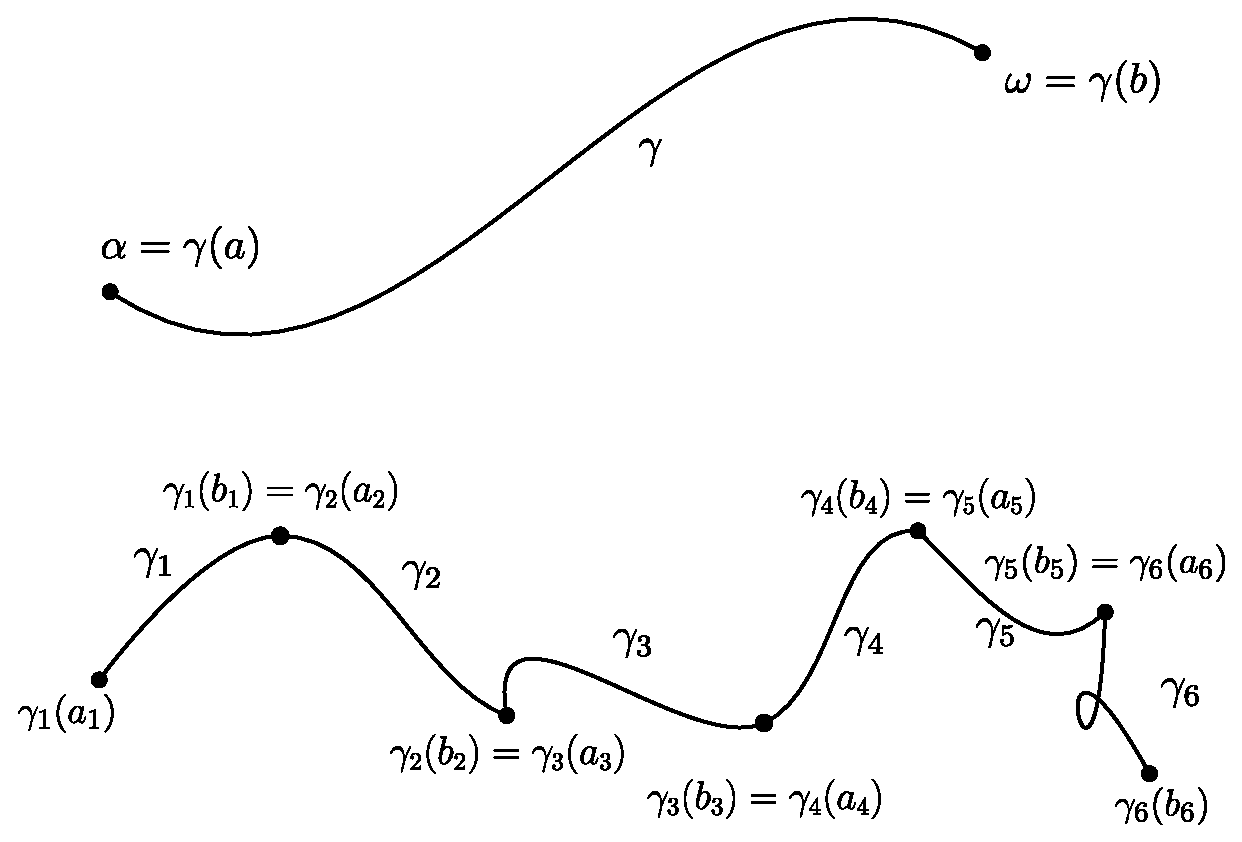
\includegraphics[scale=0.5]{Figures/Chapter3/path.eps}
    \caption{A simple path $\y$, and the path $\{\y_1, \dots, \y_6\}$.}
    \label{figure_3.1}
\end{figure}

\begin{example}\label{example_3.1}
    The path given by $\y(\th)=\cos{\th}+i\sin{\th}$, where $0 \leq \th \leq
    2\pi$ is precisely the unit sphere $S^1$.
\end{example}

\begin{lemma}\label{3.1.1}
    Let $\y$ be a simple path lying in an open set $U$, and let $f:U
    \xrightarrow{} \C$ a holomorphic function, then $f \circ \y$ is real
    differentiable with  $(f \circ \y)'(t)=(f' \circ \y)(t)\y'(t)=f'(\y(t))\y'(t)$.
\end{lemma}
\begin{proof}
    Notice that $\y:[a,b] \xrightarrow{} \C$ and $f:U \xrightarrow{} \C$, so
    that $f \circ \y:[a,b] \xrightarrow{} \C$ defines a complex valued function.
    Now, since $f$ is holomorphic, and $\y$ is of class $C^1$, they are real
    differentiable; i.e. consider the values of  $f$ and  $\y$ with imaginary
    part  $0$. Then the rest follows by the chain rule for real differentiable
    functions.
\end{proof}

\begin{figure}[h]
    \centering
    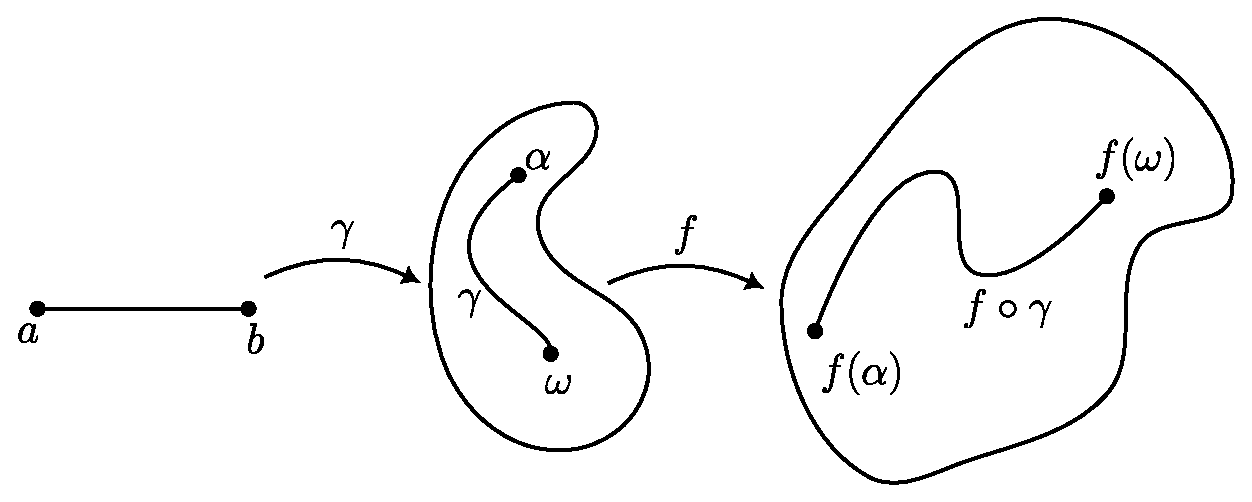
\includegraphics[scale=0.5]{Figures/Chapter3/path_composition.eps}
    \caption{The composition of a complex valued function $f$ with a simple path
     $\y_i:[a,b] \xrightarrow{} \C$.}
    \label{figure_3.2}
\end{figure}

\begin{definition}
    We define a \textbf{path} to be a sequence $\y=\{\y_i\}_{i=1}^n$ of simple
    paths such that the endpoint of the path $\y_i$ is the initial point of
    $y_{i+1}$; that is, if $\y_i$ is defined on  $[a_i,b_i]$, then
    $\y_i(b_i)=\y_{i+1}(a_{i+1})$. We call the point $\a=\y_1(a_1)$ the
    \textbf{initial point} of the path $\y$, and  $\w=\y_n(b_n)$ the \textbf{end
    point} of $\y$. We say that  $\y$  \textbf{lies} in an open set $U$ if each
    $\y_i$ lies in $U$.
\end{definition}

Figure \ref{figure_3.1} shows a simple path $\y$, and a path $\{\y_1, \dots,
\y_6\}$.

\begin{definition}
    We call an open set $U$ of $\C$ \textbf{path connected} if for every $\a, \w
    \in U$, there exists a path $\y:=\{\y_i\}_{i=1}^n$ from $\a$ to  $\w$; that
    is,  $\a$ is the initial point of $\y$, and is the end point of $\y$.
\end{definition}

\begin{theorem}\label{3.1.2}
    Let $U$ be a path connected open set, and  $f:U \xrightarrow{} \C$ a
    holomorphic function on $U$. If  $f'=0$, then $f$ is constant.
\end{theorem}
\begin{proof}
    Let $\a,\w \in U$ and let $\y:[a,b] \xrightarrow{} \C$ a simple path from
    $\a$ to  $\w$; i.e. $\a=\y(a)$ and $\w=\y(b)$. By the lemma \ref{3.1.1}, $f
    \circ \y$ is real differentiable with
    \begin{equation*}
        (f' \circ \y)(t)\y'(t)=0
    \end{equation*}
    I.e. $f \circ \y$ is constant, and  $f \circ \y(a)=f(\a)=f(\w)=f \circ
    \y(b)$. This makes $f$ constant.
\end{proof}

\begin{definition}
    If $f:U \xrightarrow{} \C$ is a complex valued function on an open set $U$
    of  $\C$, and $g$ is holomorphic on $U$ such that  $g'=f$, then we call $g$
    a \textbf{primitive} of $f$ on $U$.
\end{definition}

\begin{lemma}\label{3.1.3}
    On path connected open sets, primitives of complex valued functions are
    uniquely defined up to a constant.
\end{lemma}
\begin{proof}
    By theorem \ref{3.1.2}.
\end{proof}

\begin{example}\label{example_3.2}
    The function $f(z)=z^n$ has as primitive the function
    $g(z)=\frac{z^{n+1}}{n+1}$.
\end{example}

\begin{definition}
    Let $S$ be an arbitrary set of $\C$. We say a point $z_0 \in S$ is an
    \textbf{isolated point} in $S$ if there exists an open ball  $B(z_0,r)$,
    with $r>0$ such that $z_0$ is the only point of $S$ in  $B(z_0,r)$; that is,
    $B(z_0,r) \cap S=\{z_0\}$. We call $S$  \textbf{discrete} if every point of
    $S$ is an isolated point.
\end{definition}

\begin{theorem}\label{3.1.4}
    Let $U \subseteq \C$ be a path connected open set in  $\C$. The following
    are true for any complex valued functions  $f:U \xrightarrow{} \C$ and $g:U
    \xrightarrow{} \C$.
    \begin{enumerate}
        \item[(1)] If $f$ is analytic on  $U$, and not constant, then the set of
            zeros of  $f$ on  $U$ is discrete.

        \item[(2)] If $f$ and $g$ are analytic on $U$, and $S$ is a nondiscrete
            subset of $U$, and  $f(z)=g(z)$ for all $z \in S$, then $f=g$ on
            $U$.
    \end{enumerate}
\end{theorem}
\begin{proof}
    By theorem \ref{2.3.2}, we have that $f$ is locally constant on an open ball
    $B(z_0,r)$, with $f=0$, or  $z_0$ is an isolated point. Suppose that $f=0$
    on  $B(z_0,r)$, and let $S=\{z \in \C : f(z)=0 \text{ in } B(z_0,r)\}$. Then
    $S$ is open. Now let  $z_1 \in \cl{S}$, by the continuity of $f$, it follows
    that  $f(z_1)=0$, if $z_1 \notin S$, then there is a point arbitrarily close
    to $z_1$, and it follows that  $f=0$ locally on  $B(z_1,r)$. This makes $z_1
    \in S$ so that $S$ is closed. The second assertion follows from the first.
\end{proof}

\begin{definition}
    Let $f$ be analytic on an open set  $U$ of  $\C$, and let  $g$ be analytic
    on an open set  $V$ of  $\C$; where  $U \cap V$ is nonempty. If  $U$ and $V$
    are path connecte, and $f(z)=g(z)$ for all $z \in U \cap V$, then we call
    $g$ the  \textbf{analytic continuation} of $f$ to  $V$.
\end{definition}

\begin{theorem}[The Maximum Modulus Theorem]\label{3.1.5}
    Let $U$ be an open path connected set of $\C$, and let $f:U \xrightarrow{}
    \C$ be analytic on $U$. If  $z_0 \in U$ is a maximum for $|f|$, then  $f$ is
    constant on  $U$.
\end{theorem}
\begin{corollary}
    Let $U$ an open path connected set of $\C$, and let $f:\cl{U} \xrightarrow{} \C$
    be continuous on $U$, and analytic and nonconstant on  $U$. If  $z_0$ is a
    maxmimum for $f$ on  $\cl{U}$, then $z_0 \in \partial{(\cl{U})}$.
\end{corollary}
